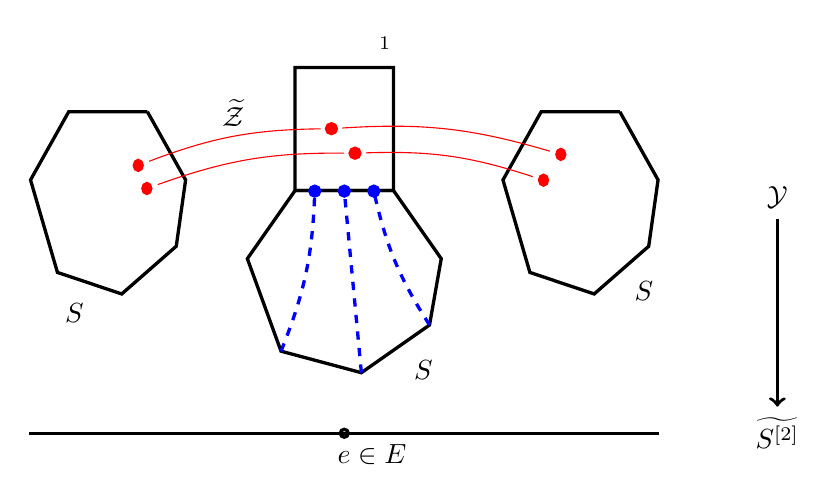
\begin{tikzpicture}[very thick]
  \draw (-4,0) -- (4,0);
  \draw (5.5, 3) node (Y) {$\mathcal Y$};
  \draw (5.5,0) node (S){$\widetilde {S^{[2]}}$};
  \draw (Y) edge[->] (S);
  \draw (0,0) circle (0.05) node [below] {$\qquad e \in E$};
  
  \begin{scope}[xshift=-3cm, yshift=3cm, yscale=1.25]
    \draw (60:1) -- (120:1) -- (170:1) -- (230:1) -- (280:1) -- (330:1) -- (10:1) -- (60:1);
    \draw[fill, red]
    (10:0.5) node (a1) {} circle (0.05)
    (40:0.5) node (a2) {} circle (0.05);
    \draw (250:1.25) node {$S$};
  \end{scope}

  \begin{scope}[xshift=3cm, yshift=3cm, yscale=1.25]
    \draw (60:1) -- (120:1) -- (170:1) -- (230:1) -- (280:1) -- (330:1) -- (10:1) -- (60:1);
    \draw[fill, red]
    (160:0.5) node (b1) {} circle (0.05)
    (120:0.5) node (b2) {} circle (0.05);
    \draw (310:1.25) node {$S$};
  \end{scope}

  \begin{scope}[yshift=2cm, scale=1.25]
    \draw (60:1) -- (120:1) -- (170:1) -- (230:1) -- (280:1) -- (330:1) -- (10:1) -- (60:1);
    \draw (60:1) -- (120:1) -- ++(0,1.25) -- ++(1,0) -- cycle;
    \draw[fill, red]
    (85:1.25) node (z1) {} circle (0.05)
    (95:1.50) node (z2) {} circle (0.05);
    \draw[blue,fill] (230:1) edge [dashed, bend right=10] (-0.3,0.86)
    (-0.3,0.86) circle (0.05);
    \draw[blue,fill] (280:1) edge [dashed] (0,0.86)
    (0,0.86) circle (0.05);
    \draw[blue,fill] (330:1) edge [dashed, bend left=10] (0.3,0.86)
    (0.3,0.86) circle (0.05);
    \draw (310:1.25) node {$S$};
    \draw (80:2.4) node {$\F_1$};
  \end{scope}
  \draw[thin, draw=red, bend left=10] (a1) edge (z1) (z1) edge (b1);
  \draw[thin, draw=red, bend left=10] (a2) edge node[above] {$\widetilde{\mathcal Z}$} (z2)
  (z2) edge (b2);
\end{tikzpicture}


%%% Local Variables:
%%% mode: latex
%%% TeX-master: "../main"
%%% End:
